\section{Results}
\label{SECIV}\label{sec:results}

In this section we test our implementation of the \lloid\ method using the
pipeline described in the previous section.  We answer the following questions
%
I) What is the measured loss of \SNR\ due to the approximations used in the
\lloid\ algorithm in a realistic analysis pipeline?
%
II) What is the measured latency of the implementation described in section
\ref{sec:implementation}?
%
III) What is the measured computational cost of the implementation described in
section \ref{sec:implementation}?

\subsection{Measured \SNR\ loss}

We expect two contributions to the \SNR\ loss to arise in our implementation of
the \lloid\ algorithm.  The first is the \SNR\ loss due to the truncation of
the SVD basis, which is fundamental, and estimates for it
exist~\cite{Cannon:2010p10398}.  The second comes from non ideal
implementations of resampling that cause signal loss.  We have measured the
effect of the resampling in the pipeline alone on a single waveform to gauge
the magnitude of the loss.  It is shown in figure \ref{fig:resamp_mm} as a
function of the quality of the {\tt audioresample} element (which is
proportional to the filter length used).  In both cases we have to compare the
\SNR\ loss to the expected \SNR\ loss that arises from the discreteness of the
template bank which is typically $\sim 3\%$.  We will consider a comparable
\SNR\ loss to be tolerable, but ideally would like to have a factor of 10 lower
loss from the \lloid\ implementation (i.e. no more than $\sim 0.3 \%$).  
%
\begin{figure}
	\label{fig:hist-interpolate}
	\begin{center}
		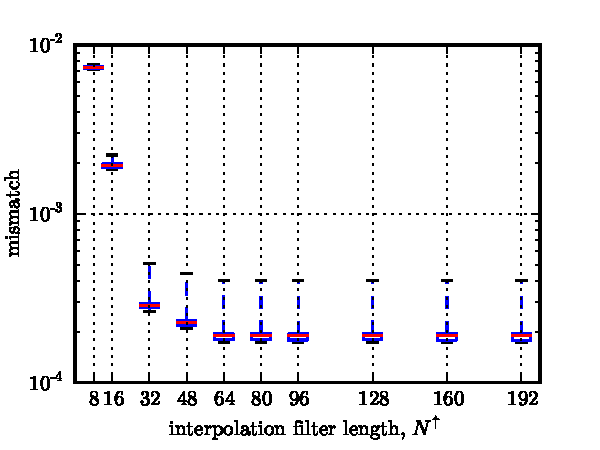
\includegraphics{bw_resample.pdf}
		\caption{Box-and-whisker plot of mismatch between nominal template bank and \lloid\ measured impulse respones.  The length $N^\shortuparrow$ of the interpolation filter is varied from 8 to 192.  The \textsc{svd} tolerance is kept fixed at $(1-10^{-6})$.  The lines in the center of the boxes denote the medians.  The upper and lower boundaries of the boxes show the upper and lower quartiles.  The whiskers denote the minimum and maximum mismatch over all templates.}
	\end{center}
\end{figure}

\begin{figure}
	\label{fig:hist-svd-tolerance}
	\begin{center}
		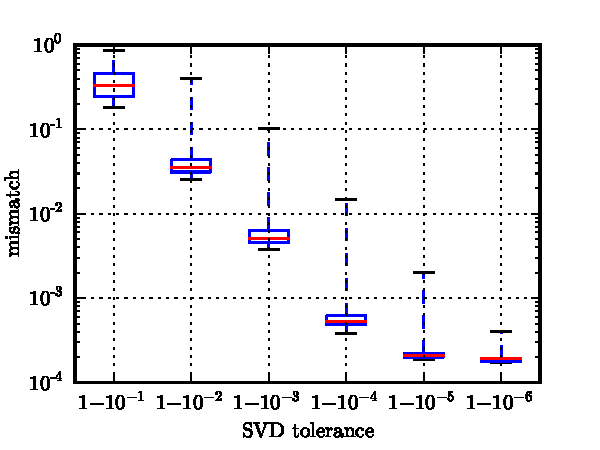
\includegraphics{bw.pdf}
		\caption{Box-and-whisker plot of mismatch between nominal
template bank and \lloid\ measured impulse respones.  The \textsc{svd}
tolerance is varied from $\left(1-10^{-1}\right)$ to $\left(1-10^{-6}\right)$.
The diminishing improvement is caused by hitting the resampling match limit.}
	\end{center}
\end{figure}


\subsection{Measured latency}

In order to check the latency of our implementation of the \lloid\ algorithm we
used the pipeline described in \ref{fig:pipeline} with a live source connected
to the input.  We then measured the timestamp of the live source and the output
of the final \SNR\ time series.  Since \gstreamer\ is not a
sample-in-sample-out realtime infrastructure, it does work by passing small
buffers of data and filtered data through the pipeline.  We set the buffer size
on the input to be 1/4 s.  In an ideal case the latency should be nearly 1/4 s.
However, it is necessary to queue things in the pipeline to assure that there
are no issues with threading. Sometimes buffers get delayed.  We measured the
average filtering latency to be \FIXME{1 s}.

\subsection{Measured computational cost}

Using the pipeline described previously, we also measured the computational
cost.  We used an 8 socket, quad core AMD\texttrademark\ machine operating at
2.7 GHz per core.  We found that filtering \FIXME{657} templates in real time
required about \FIXME{6} of the available cores.  We thus conclude that we
require about 1 core for every \FIXME{100} templates.  We note that this is
well within the computational limits of a modern, computing cluster assuming
that the scaling holds for the entire mass range of interest, we would need
about \FIXME{300} cores per detector.  This requirment should be even less of a
burden in the advanced detecor era, when presumably clusters built in that era
will have a factor of 4 or 8 more cores than the ones today. 

